\subsection{Capítulo 4: Problema 2}
Si $f$ es un mapeo continuo de un espacio métrico $X$ en un espacio métrico $Y$, pruebe que: 
$$f(\overline{E})\subset\overline{f(E)}$$
para cada conjunto $E\subset X$. ($\overline{E}$ denota la cerradura de $E$.) Muestre, con un ejemplo, $f(\overline{E})$ puede ser un subconjunto propio de $\overline{f(E)}$.

\begin{tcolorbox}[colback=gray!15,colframe=gray!1!gray,title=  Teorema 4.8 de \cite{rudin1976principles} ]
Un mapeo $f$ de un espacio métrico $X$ en un espacio métrico $Y$ es continuo en $X$ si y solo si $f^{-1}(V)$ es abierto en $X$ para cada conjunto abierto $V$ en $Y$.
\newline 

\textbf{Corolario}
\newline 
Un mapeo de un espacio métrico $X$ en un espacio métrico $Y$ es continuo si y solo si $f^{-1}(C)$ es cerrado en $X$ para cada conjunto cerrado $C$ en $Y$.
\end{tcolorbox}
\begin{tcolorbox}[colback=blue!15,colframe=blue!1!blue,title= Definición 1.3 de \cite{rudin1976principles} ]
Si $A$ y $B$ son conjuntos y si cada elemento de $A$ es un elemento de $B$, decimos que $A$ es un subconjunto de $B$, y escribimos $A\subset B$. Si, adicionalmente, hay un elemento de $B$ que no está en $A$, entonces se dice que $A$ es un conjunto propio de $B$.
\end{tcolorbox}
\begin{tcolorbox}[colback=blue!15,colframe=blue!1!blue,title= Definición 2.2 de \cite{rudin1976principles} ]
Sean $A$ y $B$ dos conjuntos y sea $f$ un mapeo de $A$ a $B$. Si $E\subset B$, $f^{-1}$ denota el conjunto de todos los $x\in A$ tales que $f(x)\in E$. Llamamos $f^{-1}$ la \textit{imagen inversa} de $E$ bajo $f$. Si $y\in B, f^{-1}(y)$ es el conjunto de todos los $x\in A$ tales que $f(x)=y$. 
\end{tcolorbox}
\begin{tcolorbox}[colback=blue!15,colframe=blue!1!blue,title= Definición (Cerradura) de \cite{rudin1976principles}]
Si $X$ es un espacio métrico, si $E\subset X$, y si $E'$ denota el conjunto de todos los puntos límites de $E$ en $X$, entonces la cerradura de $E$ es el conjunto $\overline{E}=E\cup E'$.
\end{tcolorbox}
\begin{tcolorbox}[colback=blue!15,colframe=blue!1!blue,title= Definición (Punto de acumulación) de \cite{rudin1976principles}]
Sea $X$ un espacio métrico y $E\subset X$. 
Un punto $p$ es un punto de acumulación del subconjunto $E$ si cada vecindad de $p$ contiene un punto $q\neq p$ tal que $q\in E$.
\end{tcolorbox}
\begin{tcolorbox}[colback=gray!15,colframe=gray!1!gray,title=  Teorema 3.2.12 de \cite{abbott2012understanding} ]
Para cualquier $A\subseteq \mathbb{R}$, la cerradura $\overline{A}$ es un conjunto cerrado y es el conjunto más pequeño que contiene a $A$.
\end{tcolorbox}
\begin{proof}
Por hipótesis, tenemos un mapeo continuo $f: X\to Y$, para cada conjunto $E\subset X$. A probar: $f(\overline{E})\subset \overline{f(E)}$. Gráficamente, tenemos: 
\begin{center}
    

\tikzset{every picture/.style={line width=0.75pt}} %set default line width to 0.75pt        

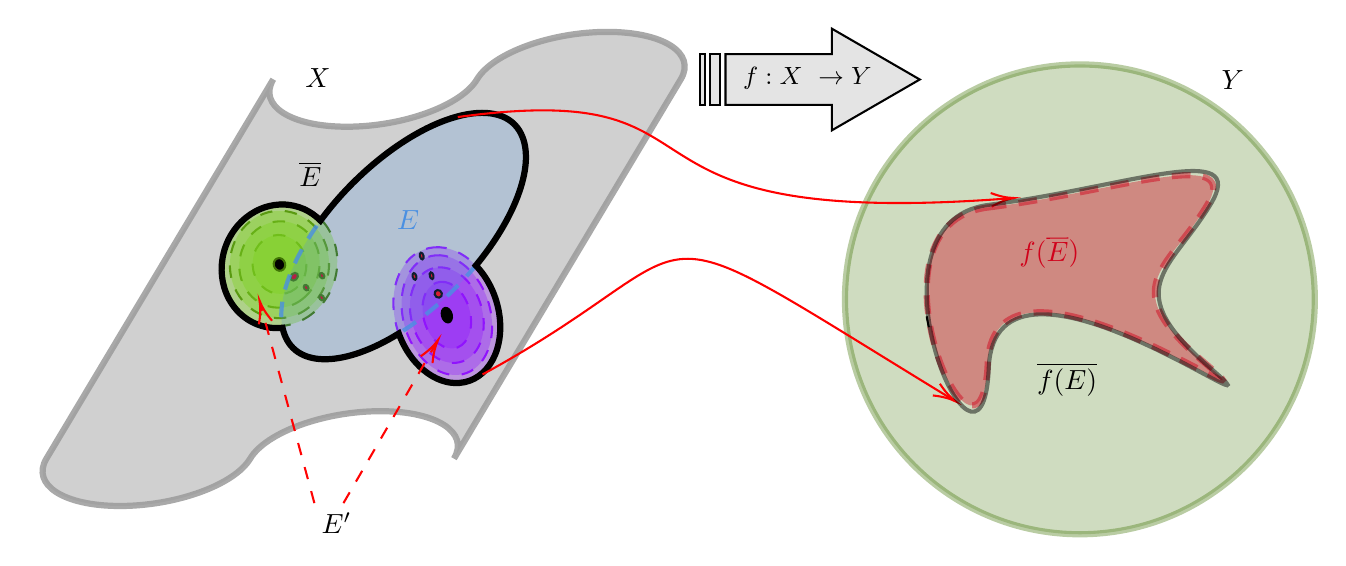
\begin{tikzpicture}[x=0.75pt,y=0.75pt,yscale=-1,xscale=1]
%uncomment if require: \path (0,300); %set diagram left start at 0, and has height of 300

%Flowchart: Punched Tape [id:dp2063300644919147] 
\draw  [color={rgb, 255:red, 155; green, 155; blue, 155 }  ,draw opacity=0.86 ][fill={rgb, 255:red, 155; green, 155; blue, 155 }  ,fill opacity=0.47 ][line width=2.25]  (127.62,40.38) .. controls (120.07,52.99) and (135.93,63.22) .. (163.04,63.22) .. controls (190.15,63.22) and (218.24,52.99) .. (225.78,40.38) .. controls (233.33,27.76) and (261.42,17.53) .. (288.53,17.53) .. controls (315.64,17.53) and (331.5,27.76) .. (323.95,40.38) -- (214.68,223.11) .. controls (222.22,210.5) and (206.36,200.27) .. (179.25,200.27) .. controls (152.14,200.27) and (124.05,210.5) .. (116.51,223.11) .. controls (108.96,235.73) and (80.87,245.95) .. (53.76,245.95) .. controls (26.65,245.95) and (10.79,235.73) .. (18.34,223.11) -- cycle ;
%Shape: Ellipse [id:dp6744338457557195] 
\draw  [color={rgb, 255:red, 144; green, 19; blue, 254 }  ,draw opacity=1 ][fill={rgb, 255:red, 144; green, 19; blue, 254 }  ,fill opacity=0.31 ][dash pattern={on 4.5pt off 4.5pt}] (208.24,137.94) .. controls (214.49,137.44) and (220.89,144.24) .. (222.54,153.1) .. controls (224.2,161.97) and (220.48,169.56) .. (214.23,170.05) .. controls (207.99,170.54) and (201.59,163.75) .. (199.93,154.88) .. controls (198.28,146.01) and (202,138.43) .. (208.24,137.94) -- cycle ;
%Shape: Ellipse [id:dp7976020204949336] 
\draw  [color={rgb, 255:red, 144; green, 19; blue, 254 }  ,draw opacity=1 ][fill={rgb, 255:red, 144; green, 19; blue, 254 }  ,fill opacity=0.31 ][dash pattern={on 4.5pt off 4.5pt}] (206.95,131.02) .. controls (216.49,130.27) and (226.13,139.94) .. (228.5,152.63) .. controls (230.87,165.32) and (225.05,176.22) .. (215.52,176.97) .. controls (205.99,177.72) and (196.34,168.04) .. (193.98,155.35) .. controls (191.61,142.66) and (197.42,131.77) .. (206.95,131.02) -- cycle ;
%Shape: Ellipse [id:dp24571623506166163] 
\draw  [color={rgb, 255:red, 144; green, 19; blue, 254 }  ,draw opacity=1 ][fill={rgb, 255:red, 144; green, 19; blue, 254 }  ,fill opacity=0.31 ][dash pattern={on 4.5pt off 4.5pt}] (205.87,125.18) .. controls (217.54,124.26) and (229.41,136.42) .. (232.38,152.33) .. controls (235.35,168.24) and (228.29,181.89) .. (216.61,182.8) .. controls (204.93,183.72) and (193.06,171.57) .. (190.1,155.66) .. controls (187.13,139.74) and (194.19,126.1) .. (205.87,125.18) -- cycle ;
%Shape: Ellipse [id:dp7029600062996805] 
\draw  [color={rgb, 255:red, 144; green, 19; blue, 254 }  ,draw opacity=1 ][fill={rgb, 255:red, 144; green, 19; blue, 254 }  ,fill opacity=0.31 ][dash pattern={on 4.5pt off 4.5pt}] (205.15,121.32) .. controls (218.96,120.23) and (232.89,133.98) .. (236.25,152.02) .. controls (239.62,170.07) and (231.14,185.58) .. (217.33,186.66) .. controls (203.51,187.75) and (189.59,174.01) .. (186.22,155.96) .. controls (182.86,137.92) and (191.33,122.41) .. (205.15,121.32) -- cycle ;

%Shape: Ellipse [id:dp3839588135077918] 
\draw  [fill={rgb, 255:red, 0; green, 0; blue, 0 }  ,fill opacity=1 ] (213.59,153.61) .. controls (213.14,151.69) and (211.73,150.3) .. (210.44,150.51) .. controls (209.14,150.72) and (208.45,152.45) .. (208.89,154.38) .. controls (209.33,156.3) and (210.74,157.69) .. (212.04,157.48) .. controls (213.33,157.26) and (214.03,155.53) .. (213.59,153.61) -- cycle ;
%Shape: Ellipse [id:dp2127132380789365] 
\draw  [fill={rgb, 255:red, 255; green, 0; blue, 0 }  ,fill opacity=1 ] (200.01,125.37) .. controls (199.8,124.48) and (199.25,123.82) .. (198.77,123.9) .. controls (198.28,123.98) and (198.06,124.76) .. (198.26,125.65) .. controls (198.47,126.54) and (199.02,127.2) .. (199.51,127.12) .. controls (199.99,127.04) and (200.21,126.26) .. (200.01,125.37) -- cycle ;
%Shape: Ellipse [id:dp8513481328263457] 
\draw  [fill={rgb, 255:red, 255; green, 0; blue, 0 }  ,fill opacity=1 ] (196.54,135.21) .. controls (196.33,134.32) and (195.78,133.66) .. (195.3,133.74) .. controls (194.81,133.82) and (194.59,134.6) .. (194.79,135.49) .. controls (195,136.38) and (195.55,137.04) .. (196.04,136.96) .. controls (196.52,136.88) and (196.74,136.1) .. (196.54,135.21) -- cycle ;
%Shape: Ellipse [id:dp8025970423246098] 
\draw  [fill={rgb, 255:red, 255; green, 0; blue, 0 }  ,fill opacity=1 ] (204.77,134.85) .. controls (204.57,133.96) and (204.01,133.3) .. (203.53,133.38) .. controls (203.05,133.46) and (202.82,134.25) .. (203.03,135.14) .. controls (203.23,136.02) and (203.79,136.68) .. (204.27,136.6) .. controls (204.75,136.52) and (204.98,135.74) .. (204.77,134.85) -- cycle ;
%Shape: Ellipse [id:dp325431177683269] 
\draw  [fill={rgb, 255:red, 255; green, 0; blue, 0 }  ,fill opacity=1 ] (205.41,144.02) .. controls (205.17,143.01) and (205.75,142.06) .. (206.69,141.91) .. controls (207.63,141.75) and (208.59,142.45) .. (208.82,143.46) .. controls (209.05,144.47) and (208.48,145.42) .. (207.53,145.57) .. controls (206.59,145.72) and (205.64,145.03) .. (205.41,144.02) -- cycle ;

%Shape: Ellipse [id:dp3401892873666933] 
\draw  [color={rgb, 255:red, 65; green, 117; blue, 5 }  ,draw opacity=1 ][fill={rgb, 255:red, 126; green, 211; blue, 33 }  ,fill opacity=0.4 ][dash pattern={on 4.5pt off 4.5pt}] (138.47,141.14) .. controls (132.78,145.7) and (124.64,144.22) .. (120.29,137.83) .. controls (115.95,131.45) and (117.04,122.58) .. (122.73,118.02) .. controls (128.43,113.46) and (136.57,114.95) .. (140.91,121.33) .. controls (145.26,127.72) and (144.17,136.59) .. (138.47,141.14) -- cycle ;
%Shape: Ellipse [id:dp17494380717696123] 
\draw  [color={rgb, 255:red, 65; green, 117; blue, 5 }  ,draw opacity=1 ][fill={rgb, 255:red, 126; green, 211; blue, 33 }  ,fill opacity=0.4 ][dash pattern={on 4.5pt off 4.5pt}] (141.86,146.13) .. controls (133.17,153.08) and (121.08,151.32) .. (114.86,142.18) .. controls (108.64,133.04) and (110.65,120) .. (119.34,113.04) .. controls (128.04,106.08) and (140.13,107.85) .. (146.35,116.98) .. controls (152.56,126.12) and (150.56,139.17) .. (141.86,146.13) -- cycle ;
%Shape: Ellipse [id:dp2837372218555473] 
\draw  [color={rgb, 255:red, 65; green, 117; blue, 5 }  ,draw opacity=1 ][fill={rgb, 255:red, 126; green, 211; blue, 33 }  ,fill opacity=0.4 ][dash pattern={on 4.5pt off 4.5pt}] (144.72,150.33) .. controls (134.07,158.85) and (119.12,156.47) .. (111.32,145.01) .. controls (103.52,133.56) and (105.83,117.36) .. (116.48,108.84) .. controls (127.13,100.32) and (142.09,102.69) .. (149.88,114.15) .. controls (157.68,125.61) and (155.37,141.8) .. (144.72,150.33) -- cycle ;
%Shape: Ellipse [id:dp15195927292003908] 
\draw  [color={rgb, 255:red, 65; green, 117; blue, 5 }  ,draw opacity=1 ][fill={rgb, 255:red, 126; green, 211; blue, 33 }  ,fill opacity=0.4 ][dash pattern={on 4.5pt off 4.5pt}] (146.61,153.11) .. controls (134.01,163.19) and (116.63,160.83) .. (107.79,147.84) .. controls (98.95,134.85) and (101.99,116.14) .. (114.59,106.06) .. controls (127.19,95.97) and (144.57,98.33) .. (153.42,111.32) .. controls (162.26,124.32) and (159.21,143.02) .. (146.61,153.11) -- cycle ;

%Shape: Ellipse [id:dp35934378533819344] 
\draw  [color={rgb, 255:red, 65; green, 117; blue, 5 }  ,draw opacity=1 ][fill={rgb, 255:red, 0; green, 0; blue, 0 }  ,fill opacity=1 ] (128.52,131.46) .. controls (129.54,132.79) and (131.3,133.03) .. (132.45,131.99) .. controls (133.6,130.95) and (133.7,129.03) .. (132.68,127.7) .. controls (131.66,126.37) and (129.9,126.13) .. (128.75,127.17) .. controls (127.61,128.21) and (127.5,130.13) .. (128.52,131.46) -- cycle ;
%Shape: Ellipse [id:dp9594760206814382] 
\draw  [color={rgb, 255:red, 65; green, 117; blue, 5 }  ,draw opacity=1 ][fill={rgb, 255:red, 208; green, 2; blue, 27 }  ,fill opacity=1 ] (150.16,146.28) .. controls (150.63,146.9) and (151.36,147.08) .. (151.78,146.7) .. controls (152.21,146.31) and (152.17,145.5) .. (151.7,144.89) .. controls (151.23,144.27) and (150.5,144.09) .. (150.08,144.47) .. controls (149.65,144.86) and (149.69,145.67) .. (150.16,146.28) -- cycle ;
%Shape: Ellipse [id:dp1610532202233017] 
\draw  [color={rgb, 255:red, 65; green, 117; blue, 5 }  ,draw opacity=1 ][fill={rgb, 255:red, 208; green, 2; blue, 27 }  ,fill opacity=1 ] (150.31,135.68) .. controls (150.78,136.29) and (151.51,136.48) .. (151.93,136.09) .. controls (152.36,135.71) and (152.32,134.89) .. (151.85,134.28) .. controls (151.38,133.67) and (150.65,133.48) .. (150.22,133.87) .. controls (149.8,134.25) and (149.83,135.06) .. (150.31,135.68) -- cycle ;
%Shape: Ellipse [id:dp8346680962527804] 
\draw  [color={rgb, 255:red, 65; green, 117; blue, 5 }  ,draw opacity=1 ][fill={rgb, 255:red, 208; green, 2; blue, 27 }  ,fill opacity=1 ] (142.7,141.44) .. controls (143.17,142.06) and (143.9,142.24) .. (144.33,141.86) .. controls (144.75,141.47) and (144.72,140.66) .. (144.24,140.05) .. controls (143.77,139.43) and (143.04,139.25) .. (142.62,139.63) .. controls (142.19,140.02) and (142.23,140.83) .. (142.7,141.44) -- cycle ;
%Shape: Ellipse [id:dp09099591294015819] 
\draw  [color={rgb, 255:red, 65; green, 117; blue, 5 }  ,draw opacity=1 ][fill={rgb, 255:red, 208; green, 2; blue, 27 }  ,fill opacity=1 ] (139.22,134.13) .. controls (139.75,134.83) and (139.51,136.01) .. (138.68,136.76) .. controls (137.84,137.52) and (136.73,137.56) .. (136.19,136.86) .. controls (135.66,136.16) and (135.9,134.98) .. (136.73,134.23) .. controls (137.57,133.47) and (138.68,133.43) .. (139.22,134.13) -- cycle ;

%Shape: Ellipse [id:dp5845259294408545] 
\draw  [color={rgb, 255:red, 74; green, 144; blue, 226 }  ,draw opacity=0.8 ][fill={rgb, 255:red, 74; green, 144; blue, 226 }  ,fill opacity=0.21 ][dash pattern={on 5.63pt off 4.5pt}][line width=1.5]  (247.74,68.29) .. controls (255.28,87.85) and (235.72,125.02) .. (204.05,151.31) .. controls (172.39,177.61) and (140.62,183.07) .. (133.09,163.51) .. controls (125.56,143.95) and (145.12,106.78) .. (176.78,80.48) .. controls (208.44,54.19) and (240.21,48.73) .. (247.74,68.29) -- cycle ;

%Shape: Path Data [id:dp7690042854635427] 
\draw  [color={rgb, 255:red, 0; green, 0; blue, 0 }  ,draw opacity=1 ][line width=2.25]  (236.25,152.02) .. controls (239.61,170.07) and (231.14,185.58) .. (217.33,186.66) .. controls (205.34,187.61) and (193.27,177.38) .. (188.09,162.87) .. controls (162.34,178.75) and (139.35,179.77) .. (133.1,163.52) .. controls (132.67,162.43) and (132.34,161.28) .. (132.08,160.08) .. controls (122.82,161.08) and (113.51,157.12) .. (107.79,148.71) .. controls (98.94,135.72) and (101.99,117.01) .. (114.59,106.93) .. controls (125.86,97.91) and (140.97,98.85) .. (150.36,108.45) .. controls (157.56,98.63) and (166.53,88.98) .. (176.77,80.47) .. controls (208.43,54.17) and (240.2,48.71) .. (247.74,68.28) .. controls (253.4,82.97) and (243.77,107.61) .. (225.22,130.1) .. controls (230.55,135.62) and (234.63,143.32) .. (236.25,152.02) -- cycle ;
%Shape: Ellipse [id:dp30885511353850836] 
\draw  [color={rgb, 255:red, 65; green, 117; blue, 5 }  ,draw opacity=0.37 ][fill={rgb, 255:red, 65; green, 117; blue, 5 }  ,fill opacity=0.25 ][line width=2.25]  (403.06,146.39) .. controls (403.06,83.88) and (453.74,33.21) .. (516.25,33.21) .. controls (578.75,33.21) and (629.43,83.88) .. (629.43,146.39) .. controls (629.43,208.9) and (578.75,259.57) .. (516.25,259.57) .. controls (453.74,259.57) and (403.06,208.9) .. (403.06,146.39) -- cycle ;
%Striped Right Arrow [id:dp2791040078229359] 
\draw  [fill={rgb, 255:red, 128; green, 128; blue, 128 }  ,fill opacity=0.21 ] (345.5,28.24) -- (396.77,28.24) -- (396.77,16) -- (439.1,40.47) -- (396.77,64.95) -- (396.77,52.71) -- (345.5,52.71) -- cycle ;\draw  [fill={rgb, 255:red, 128; green, 128; blue, 128 }  ,fill opacity=0.21 ] (333.26,28.24) -- (335.71,28.24) -- (335.71,52.71) -- (333.26,52.71) -- cycle ;\draw  [fill={rgb, 255:red, 128; green, 128; blue, 128 }  ,fill opacity=0.21 ] (338.15,28.24) -- (343.05,28.24) -- (343.05,52.71) -- (338.15,52.71) -- cycle ;

%Curve Lines [id:da7799398101911289] 
\draw [color={rgb, 255:red, 255; green, 0; blue, 0 }  ,draw opacity=1 ]   (216.52,58.56) .. controls (358.48,39.17) and (273.58,114.17) .. (484.43,97.57) ;
\draw [shift={(484.43,97.57)}, rotate = 535.5] [color={rgb, 255:red, 255; green, 0; blue, 0 }  ,draw opacity=1 ][line width=0.75]    (10.93,-3.29) .. controls (6.95,-1.4) and (3.31,-0.3) .. (0,0) .. controls (3.31,0.3) and (6.95,1.4) .. (10.93,3.29)   ;
%Curve Lines [id:da6918085781367213] 
\draw [color={rgb, 255:red, 255; green, 0; blue, 0 }  ,draw opacity=1 ]   (228.43,182.57) .. controls (347.94,117.31) and (291.46,95.03) .. (456.43,195.57) ;
\draw [shift={(456.43,195.57)}, rotate = 211.36] [color={rgb, 255:red, 255; green, 0; blue, 0 }  ,draw opacity=1 ][line width=0.75]    (10.93,-3.29) .. controls (6.95,-1.4) and (3.31,-0.3) .. (0,0) .. controls (3.31,0.3) and (6.95,1.4) .. (10.93,3.29)   ;
%Straight Lines [id:da28756547839686364] 
\draw [color={rgb, 255:red, 255; green, 3; blue, 3 }  ,draw opacity=1 ] [dash pattern={on 4.5pt off 4.5pt}]  (147.43,244.57) -- (121.52,148.93) ;
\draw [shift={(121,147)}, rotate = 434.84000000000003] [color={rgb, 255:red, 255; green, 3; blue, 3 }  ,draw opacity=1 ][line width=0.75]    (10.93,-3.29) .. controls (6.95,-1.4) and (3.31,-0.3) .. (0,0) .. controls (3.31,0.3) and (6.95,1.4) .. (10.93,3.29)   ;
%Straight Lines [id:da30133818771395926] 
\draw [color={rgb, 255:red, 255; green, 3; blue, 3 }  ,draw opacity=1 ] [dash pattern={on 4.5pt off 4.5pt}]  (161.43,244.57) -- (206,167.73) ;
\draw [shift={(207,166)}, rotate = 480.11] [color={rgb, 255:red, 255; green, 3; blue, 3 }  ,draw opacity=1 ][line width=0.75]    (10.93,-3.29) .. controls (6.95,-1.4) and (3.31,-0.3) .. (0,0) .. controls (3.31,0.3) and (6.95,1.4) .. (10.93,3.29)   ;
%Shape: Polygon Curved [id:ds09372127946980235] 
\draw  [color={rgb, 255:red, 208; green, 2; blue, 27 }  ,draw opacity=0.48 ][fill={rgb, 255:red, 208; green, 2; blue, 27 }  ,fill opacity=0.38 ][dash pattern={on 6.75pt off 4.5pt}][line width=2.25]  (471.84,102.15) .. controls (536.5,94.09) and (595.99,71.53) .. (576.83,102.15) .. controls (557.66,132.78) and (533,140.48) .. (576.83,177.38) .. controls (620.66,214.28) and (474.84,106.45) .. (471.84,177.38) .. controls (468.84,248.31) and (407.19,110.21) .. (471.84,102.15) -- cycle ;
%Shape: Polygon Curved [id:ds9418229537022247] 
\draw  [color={rgb, 255:red, 0; green, 0; blue, 0 }  ,draw opacity=0.48 ][line width=1.5]  (472.34,100.86) .. controls (538.08,92.44) and (598.57,68.85) .. (579.08,100.86) .. controls (559.6,132.87) and (534.52,140.91) .. (579.08,179.47) .. controls (623.64,218.03) and (475.39,105.35) .. (472.34,179.47) .. controls (469.29,253.59) and (406.59,109.28) .. (472.34,100.86) -- cycle ;
%Straight Lines [id:da6982767133378682] 
\draw    (442.43,154.59) -- (443.45,159.82) ;



% Text Node
\draw (352.52,33.18) node [anchor=north west][inner sep=0.75pt]  [font=\small]  {$f:X\ \rightarrow Y$};
% Text Node
\draw (185.82,102.12) node [anchor=north west][inner sep=0.75pt]  [color={rgb, 255:red, 74; green, 144; blue, 226 }  ,opacity=1 ]  {$E$};
% Text Node
\draw (149.43,247.79) node [anchor=north west][inner sep=0.75pt]    {$E'$};
% Text Node
\draw (141.6,33.95) node [anchor=north west][inner sep=0.75pt]    {$X$};
% Text Node
\draw (138.64,78.52) node [anchor=north west][inner sep=0.75pt]    {$\overline{E}$};
% Text Node
\draw (583,34.57) node [anchor=north west][inner sep=0.75pt]    {$Y$};
% Text Node
\draw (494.13,175.57) node [anchor=north west][inner sep=0.75pt]    {$\overline{f( E)}$};
% Text Node
\draw (485.42,114.77) node [anchor=north west][inner sep=0.75pt]  [color={rgb, 255:red, 208; green, 2; blue, 27 }  ,opacity=1 ,rotate=-359.51]  {$f(\overline{E})$};


\end{tikzpicture}
\end{center}

\begin{noter}{Nota 1}
 Como no sabemos que la función $f$ es biyectiva y por lo tanto no podemos afirmar que tiene inversa, entonces $f^{-1}$ representará a la preimagen.
\end{noter}
Por la figura anterior, notamos que $\left(\overline{f(E)}\right)^c=Y-\overline{f(E)}$, que es un abierto de $Y$.
 $\implies$ Por el corolario del teorema 4.8 de \cite{rudin1976principles}, $f^{-1}(Y-\overline{f(E)})$ es un abierto de $X$. Ahora bien, 
 \begin{align*}
     f^{-1}(Y-\overline{f(E)}) &=f^{-1}(Y)-f^{-1}\left(\overline{f(E)}\right)\\
     &= X-f^{-1}\left(\overline{f(E)}\right).
 \end{align*}
Por lo cual, concluimos que $f^{-1}\left(\overline{f(E)}\right)$ es un cerrado de $X$. 
 
\begin{noter}{Nota 2}
Sabemos por definición $E\subset \overline{E}$, en donde $\overline{E}=E'\cup E$.
\end{noter} 
 
 \begin{noter}{Nota 3}
  Supóngase que tenemos un punto $x\in E$, entonces $f(x)\in f(E)$, aplicando la preimagen tenemos $x\in f^{-1}\left(f(E)\right)$. La preimagen se define como $$f^{-1}(f(E))=\{x:f(x)\in f(E)\}.$$
  
  Entonces, por la definición de preimagen, podemos concluir que $$E\subset f^{-1}(f(E)).$$
 \end{noter}
 
 $\implies$ Nótese que ahora podemos concluir,
 $$E\subset \underbrace{f^{-1}\left(f(E)\right) \subset f^{-1}\left(\overline{f(E)}\right)}_{\text{aplicando } f(E)\subset \overline{f(E)}}.$$

\begin{noter}{Nota 4}
Hasta el momento, sabemos que $f^{-1}\left(\overline{f(E)}\right)$ es un subconjunto cerrado y que $E\subset f^{-1}\left(\overline{f(E)}\right)$. Ahora, nos interesa conocer si $$E\subset f^{-1}\left(\overline{f(E)}\right)\implies \overline{E}\subset f^{-1}\left(\overline{f(E)}\right).$$
Por el teorema 3.2.12 de \cite{abbott2012understanding}, sabemos que $\overline{E}$ es el subconjunto cerrado más pequeño que \textbf{contiene} a $E$ (i.e. $E\subset\overline{E}$). Además, como ya sabíamos, 

$$E\subset f^{-1}\left(f(E)\right) \subset f^{-1}\left(\overline{f(E)}\right).$$

Entonces, 
$$ \overline{E}\subset f^{-1}\left(\overline{f(E)}\right)$$

\begin{center}
    

\tikzset{every picture/.style={line width=0.75pt}} %set default line width to 0.75pt        

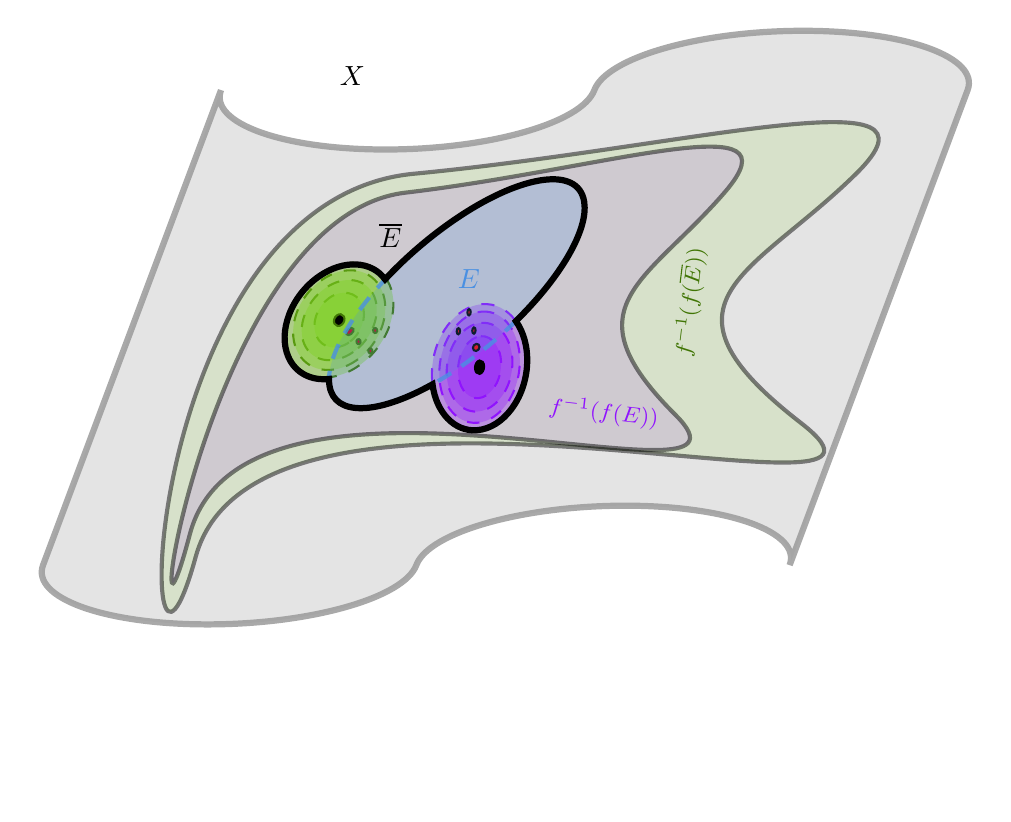
\begin{tikzpicture}[x=0.75pt,y=0.75pt,yscale=-1,xscale=1]
%uncomment if require: \path (0,300); %set diagram left start at 0, and has height of 300

%Flowchart: Punched Tape [id:dp0007829793217875025] 
\draw  [color={rgb, 255:red, 155; green, 155; blue, 155 }  ,draw opacity=0.86 ][fill={rgb, 255:red, 155; green, 155; blue, 155 }  ,fill opacity=0.27 ][line width=2.25]  (188.85,37.31) .. controls (182.93,53.11) and (218.4,65.91) .. (268.06,65.91) .. controls (317.72,65.91) and (362.78,53.11) .. (368.7,37.31) .. controls (374.62,21.52) and (419.68,8.71) .. (469.34,8.71) .. controls (519.01,8.71) and (554.47,21.52) .. (548.55,37.31) -- (462.83,266.11) .. controls (468.74,250.32) and (433.28,237.51) .. (383.62,237.51) .. controls (333.95,237.51) and (288.89,250.32) .. (282.97,266.11) .. controls (277.06,281.91) and (232,294.71) .. (182.33,294.71) .. controls (132.67,294.71) and (97.2,281.91) .. (103.12,266.11) -- cycle ;
%Shape: Polygon Curved [id:ds6101698196452915] 
\draw  [color={rgb, 255:red, 0; green, 0; blue, 0 }  ,draw opacity=0.48 ][fill={rgb, 255:red, 126; green, 211; blue, 33 }  ,fill opacity=0.13 ][line width=1.5]  (281.63,77.6) .. controls (415.76,64.73) and (544.51,28.7) .. (494.82,77.6) .. controls (445.13,126.51) and (392.34,138.81) .. (468.35,197.73) .. controls (544.37,256.65) and (207.7,148.9) .. (176.65,262.16) .. controls (145.6,375.42) and (147.5,90.47) .. (281.63,77.6) -- cycle ;

%Shape: Polygon Curved [id:ds6459300614771549] 
\draw  [color={rgb, 255:red, 0; green, 0; blue, 0 }  ,draw opacity=0.48 ][fill={rgb, 255:red, 144; green, 19; blue, 254 }  ,fill opacity=0.11 ][line width=1.5]  (277.65,86.7) .. controls (374.86,75.23) and (469.06,43.11) .. (431.39,86.7) .. controls (393.72,130.29) and (355.19,141.25) .. (407.8,193.76) .. controls (460.41,246.27) and (200.46,150.35) .. (173.83,251.29) .. controls (147.19,352.24) and (180.44,98.17) .. (277.65,86.7) -- cycle ;

%Shape: Ellipse [id:dp5815265070804121] 
\draw  [color={rgb, 255:red, 144; green, 19; blue, 254 }  ,draw opacity=1 ][fill={rgb, 255:red, 144; green, 19; blue, 254 }  ,fill opacity=0.31 ][dash pattern={on 4.5pt off 4.5pt}] (314.01,155.87) .. controls (319.73,155.41) and (324.1,161.72) .. (323.78,169.96) .. controls (323.45,178.2) and (318.54,185.25) .. (312.82,185.71) .. controls (307.1,186.16) and (302.73,179.85) .. (303.06,171.61) .. controls (303.38,163.37) and (308.29,156.32) .. (314.01,155.87) -- cycle ;
%Shape: Ellipse [id:dp4878452214127891] 
\draw  [color={rgb, 255:red, 144; green, 19; blue, 254 }  ,draw opacity=1 ][fill={rgb, 255:red, 144; green, 19; blue, 254 }  ,fill opacity=0.31 ][dash pattern={on 4.5pt off 4.5pt}] (314.27,149.44) .. controls (323,148.74) and (329.71,157.74) .. (329.24,169.53) .. controls (328.77,181.32) and (321.3,191.44) .. (312.57,192.14) .. controls (303.83,192.83) and (297.13,183.84) .. (297.6,172.04) .. controls (298.07,160.25) and (305.53,150.13) .. (314.27,149.44) -- cycle ;
%Shape: Ellipse [id:dp7551467515793162] 
\draw  [color={rgb, 255:red, 144; green, 19; blue, 254 }  ,draw opacity=1 ][fill={rgb, 255:red, 144; green, 19; blue, 254 }  ,fill opacity=0.31 ][dash pattern={on 4.5pt off 4.5pt}] (314.48,144.01) .. controls (325.18,143.16) and (333.38,154.46) .. (332.79,169.24) .. controls (332.2,184.03) and (323.05,196.71) .. (312.35,197.56) .. controls (301.65,198.41) and (293.45,187.11) .. (294.04,172.33) .. controls (294.63,157.54) and (303.78,144.87) .. (314.48,144.01) -- cycle ;
%Shape: Ellipse [id:dp9481319866996253] 
\draw  [color={rgb, 255:red, 144; green, 19; blue, 254 }  ,draw opacity=1 ][fill={rgb, 255:red, 144; green, 19; blue, 254 }  ,fill opacity=0.31 ][dash pattern={on 4.5pt off 4.5pt}] (314.63,140.43) .. controls (327.29,139.42) and (337.01,152.19) .. (336.34,168.96) .. controls (335.67,185.73) and (324.87,200.14) .. (312.21,201.15) .. controls (299.55,202.15) and (289.82,189.38) .. (290.49,172.61) .. controls (291.16,155.84) and (301.96,141.43) .. (314.63,140.43) -- cycle ;

%Shape: Ellipse [id:dp9014659043411422] 
\draw  [fill={rgb, 255:red, 0; green, 0; blue, 0 }  ,fill opacity=1 ] (315.61,170.43) .. controls (315.61,168.64) and (314.62,167.35) .. (313.41,167.55) .. controls (312.2,167.75) and (311.22,169.36) .. (311.22,171.14) .. controls (311.23,172.93) and (312.21,174.22) .. (313.42,174.02) .. controls (314.64,173.82) and (315.61,172.22) .. (315.61,170.43) -- cycle ;
%Shape: Ellipse [id:dp5055542881473339] 
\draw  [fill={rgb, 255:red, 255; green, 0; blue, 0 }  ,fill opacity=1 ] (309.16,144.19) .. controls (309.16,143.36) and (308.8,142.75) .. (308.35,142.83) .. controls (307.9,142.9) and (307.53,143.63) .. (307.53,144.46) .. controls (307.54,145.28) and (307.9,145.89) .. (308.35,145.82) .. controls (308.8,145.74) and (309.17,145.02) .. (309.16,144.19) -- cycle ;
%Shape: Ellipse [id:dp5149622164559918] 
\draw  [fill={rgb, 255:red, 255; green, 0; blue, 0 }  ,fill opacity=1 ] (304.02,153.33) .. controls (304.02,152.51) and (303.66,151.9) .. (303.21,151.97) .. controls (302.76,152.04) and (302.39,152.77) .. (302.39,153.6) .. controls (302.4,154.42) and (302.76,155.03) .. (303.21,154.96) .. controls (303.66,154.89) and (304.03,154.16) .. (304.02,153.33) -- cycle ;
%Shape: Ellipse [id:dp2571372561778966] 
\draw  [fill={rgb, 255:red, 255; green, 0; blue, 0 }  ,fill opacity=1 ] (311.51,153) .. controls (311.51,152.18) and (311.14,151.57) .. (310.69,151.64) .. controls (310.24,151.71) and (309.88,152.44) .. (309.88,153.27) .. controls (309.89,154.09) and (310.25,154.7) .. (310.7,154.63) .. controls (311.15,154.56) and (311.51,153.83) .. (311.51,153) -- cycle ;
%Shape: Ellipse [id:dp7629728082265976] 
\draw  [fill={rgb, 255:red, 255; green, 0; blue, 0 }  ,fill opacity=1 ] (310.21,161.52) .. controls (310.2,160.58) and (310.92,159.7) .. (311.8,159.56) .. controls (312.68,159.41) and (313.39,160.06) .. (313.39,161) .. controls (313.4,161.94) and (312.68,162.82) .. (311.8,162.96) .. controls (310.92,163.1) and (310.21,162.46) .. (310.21,161.52) -- cycle ;

%Shape: Ellipse [id:dp7763379887029782] 
\draw  [color={rgb, 255:red, 65; green, 117; blue, 5 }  ,draw opacity=1 ][fill={rgb, 255:red, 126; green, 211; blue, 33 }  ,fill opacity=0.4 ][dash pattern={on 4.5pt off 4.5pt}] (250.52,158.85) .. controls (244.45,163.08) and (237.42,161.7) .. (234.82,155.77) .. controls (232.21,149.84) and (235.01,141.6) .. (241.07,137.36) .. controls (247.13,133.13) and (254.16,134.51) .. (256.77,140.44) .. controls (259.38,146.37) and (256.58,154.61) .. (250.52,158.85) -- cycle ;
%Shape: Ellipse [id:dp564993296395887] 
\draw  [color={rgb, 255:red, 65; green, 117; blue, 5 }  ,draw opacity=1 ][fill={rgb, 255:red, 126; green, 211; blue, 33 }  ,fill opacity=0.4 ][dash pattern={on 4.5pt off 4.5pt}] (252.55,163.48) .. controls (243.29,169.94) and (232.76,168.3) .. (229.03,159.81) .. controls (225.3,151.32) and (229.78,139.2) .. (239.04,132.74) .. controls (248.29,126.27) and (258.82,127.91) .. (262.55,136.4) .. controls (266.29,144.89) and (261.81,157.01) .. (252.55,163.48) -- cycle ;
%Shape: Ellipse [id:dp5773899392859461] 
\draw  [color={rgb, 255:red, 65; green, 117; blue, 5 }  ,draw opacity=1 ][fill={rgb, 255:red, 126; green, 211; blue, 33 }  ,fill opacity=0.4 ][dash pattern={on 4.5pt off 4.5pt}] (254.27,167.38) .. controls (242.93,175.3) and (229.94,173.09) .. (225.27,162.44) .. controls (220.59,151.8) and (225.98,136.75) .. (237.32,128.83) .. controls (248.66,120.91) and (261.64,123.13) .. (266.32,133.77) .. controls (271,144.41) and (265.6,159.46) .. (254.27,167.38) -- cycle ;
%Shape: Ellipse [id:dp8573796123683731] 
\draw  [color={rgb, 255:red, 65; green, 117; blue, 5 }  ,draw opacity=1 ][fill={rgb, 255:red, 126; green, 211; blue, 33 }  ,fill opacity=0.4 ][dash pattern={on 4.5pt off 4.5pt}] (255.4,169.96) .. controls (241.99,179.33) and (226.81,177.14) .. (221.5,165.07) .. controls (216.2,153) and (222.77,135.62) .. (236.19,126.25) .. controls (249.6,116.88) and (264.78,119.07) .. (270.08,131.14) .. controls (275.39,143.21) and (268.82,160.59) .. (255.4,169.96) -- cycle ;

%Shape: Ellipse [id:dp7264393226887292] 
\draw  [color={rgb, 255:red, 65; green, 117; blue, 5 }  ,draw opacity=1 ][fill={rgb, 255:red, 0; green, 0; blue, 0 }  ,fill opacity=1 ] (243.54,149.85) .. controls (244.18,151.09) and (245.72,151.31) .. (246.97,150.34) .. controls (248.21,149.38) and (248.7,147.59) .. (248.05,146.36) .. controls (247.4,145.12) and (245.87,144.9) .. (244.62,145.87) .. controls (243.37,146.84) and (242.89,148.62) .. (243.54,149.85) -- cycle ;
%Shape: Ellipse [id:dp3862048882872069] 
\draw  [color={rgb, 255:red, 65; green, 117; blue, 5 }  ,draw opacity=1 ][fill={rgb, 255:red, 208; green, 2; blue, 27 }  ,fill opacity=1 ] (259.99,163.62) .. controls (260.29,164.19) and (260.9,164.37) .. (261.37,164.01) .. controls (261.83,163.65) and (261.96,162.89) .. (261.66,162.32) .. controls (261.36,161.75) and (260.75,161.58) .. (260.28,161.94) .. controls (259.82,162.3) and (259.69,163.05) .. (259.99,163.62) -- cycle ;
%Shape: Ellipse [id:dp4444721618380525] 
\draw  [color={rgb, 255:red, 65; green, 117; blue, 5 }  ,draw opacity=1 ][fill={rgb, 255:red, 208; green, 2; blue, 27 }  ,fill opacity=1 ] (262.29,153.77) .. controls (262.59,154.34) and (263.21,154.51) .. (263.67,154.15) .. controls (264.13,153.8) and (264.27,153.04) .. (263.97,152.47) .. controls (263.67,151.9) and (263.05,151.73) .. (262.59,152.09) .. controls (262.12,152.45) and (261.99,153.2) .. (262.29,153.77) -- cycle ;
%Shape: Ellipse [id:dp567119539887381] 
\draw  [color={rgb, 255:red, 65; green, 117; blue, 5 }  ,draw opacity=1 ][fill={rgb, 255:red, 208; green, 2; blue, 27 }  ,fill opacity=1 ] (254.26,159.13) .. controls (254.56,159.7) and (255.18,159.87) .. (255.64,159.51) .. controls (256.1,159.15) and (256.24,158.4) .. (255.94,157.83) .. controls (255.64,157.26) and (255.02,157.08) .. (254.56,157.44) .. controls (254.09,157.8) and (253.96,158.56) .. (254.26,159.13) -- cycle ;
%Shape: Ellipse [id:dp38180923109521825] 
\draw  [color={rgb, 255:red, 65; green, 117; blue, 5 }  ,draw opacity=1 ][fill={rgb, 255:red, 208; green, 2; blue, 27 }  ,fill opacity=1 ] (252.62,152.33) .. controls (252.96,152.98) and (252.5,154.07) .. (251.6,154.78) .. controls (250.69,155.48) and (249.68,155.52) .. (249.34,154.87) .. controls (249,154.22) and (249.46,153.13) .. (250.36,152.42) .. controls (251.27,151.72) and (252.28,151.68) .. (252.62,152.33) -- cycle ;

%Shape: Ellipse [id:dp17681093657023306] 
\draw  [color={rgb, 255:red, 74; green, 144; blue, 226 }  ,draw opacity=0.8 ][fill={rgb, 255:red, 74; green, 144; blue, 226 }  ,fill opacity=0.21 ][dash pattern={on 5.63pt off 4.5pt}][line width=1.5]  (363.84,91.14) .. controls (366.62,109.32) and (341.39,143.88) .. (307.49,168.32) .. controls (273.59,192.76) and (243.86,197.83) .. (241.08,179.65) .. controls (238.31,161.46) and (263.54,126.91) .. (297.44,102.47) .. controls (331.34,78.03) and (361.07,72.96) .. (363.84,91.14) -- cycle ;


%Shape: Path Data [id:dp8495538675132187] 
\draw  [color={rgb, 255:red, 0; green, 0; blue, 0 }  ,draw opacity=1 ][line width=2.25]  (336.35,168.96) .. controls (335.68,185.72) and (324.87,200.13) .. (312.21,201.14) .. controls (301.22,202.02) and (292.44,192.51) .. (290.75,179.03) .. controls (264.3,193.79) and (243.4,194.73) .. (241.09,179.63) .. controls (240.93,178.62) and (240.86,177.56) .. (240.88,176.44) .. controls (232.33,177.37) and (224.76,173.69) .. (221.32,165.88) .. controls (216.02,153.81) and (222.59,136.43) .. (236.01,127.06) .. controls (248.01,118.68) and (261.42,119.55) .. (267.91,128.47) .. controls (276.41,119.35) and (286.47,110.38) .. (297.43,102.48) .. controls (331.33,78.05) and (361.06,72.97) .. (363.84,91.15) .. controls (365.93,104.8) and (352.22,127.69) .. (330.9,148.59) .. controls (334.57,153.72) and (336.67,160.87) .. (336.35,168.96) -- cycle ;



% Text Node
\draw (244.64,24.58) node [anchor=north west][inner sep=0.75pt]    {$X$};
% Text Node
\draw (263.7,99.97) node [anchor=north west][inner sep=0.75pt]    {$\overline{E}$};
% Text Node
\draw (301.42,122.04) node [anchor=north west][inner sep=0.75pt]  [color={rgb, 255:red, 74; green, 144; blue, 226 }  ,opacity=1 ]  {$E$};
% Text Node
\draw (346.21,182.37) node [anchor=north west][inner sep=0.75pt]  [font=\footnotesize,color={rgb, 255:red, 144; green, 19; blue, 254 }  ,opacity=1 ,rotate=-6.38]  {$f^{-1}( f( E))$};
% Text Node
\draw (403.3,166.45) node [anchor=north west][inner sep=0.75pt]  [font=\footnotesize,color={rgb, 255:red, 65; green, 117; blue, 5 }  ,opacity=1 ,rotate=-276.97]  {$f^{-1}( f(\overline{E}))$};


\end{tikzpicture}
\end{center}
\end{noter}

Por lo tanto, 
\begin{align*}
    \overline{E}&\subset f^{-1}\left(\overline{f(E)}\right)\\
    f\left(\overline{E}\right)&\subset f\left( f^{-1}\left(\overline{f(E)}\right)\right)\\
    f\left(\overline{E}\right)&\subset \overline{f(E)}
\end{align*}
\end{proof}

\newpage 
\begin{noter}{Ejemplo}
Muestre con un ejemplo, $f(\overline{E})$ puede ser un subconjunto propio de $\overline{f(E)}$.

\begin{solution}
Basándonos en la definición 1.3 de conjunto propio de \cite{rudin1976principles}. Es necesario encontrar un elemento $\overline{f(E)}$ que no está en $f(\overline{E})$, es decir que los dos conjuntos sean diferentes. Se propone una función continua definida en $f:\mathbb{N}\to \mathbb{R}$: 

$$f(x)=\frac{1}{x}, \quad \text{es ampliamente conocida que es continua.}$$

Es decir, que tenemos $E=\mathbb{N}$. En donde $\mathbb{N}:= [1,\infty)$. Por lo tanto, $E= \overline{E}= [1,\infty)$. Entonces, al aplicar el mapeo: 

$$f(\overline{E})=f(\mathbb{N})=(0,1] $$

Por lo que ahora, notamos que: 
$$\overline{f(E)}=[0,1]$$

Es decir, el $0$ está en $\overline{f(E)}$, pero no en $f(\overline{E})$. Por lo tanto, es un subconjunto propio. 
\end{solution}
\end{noter}